\subsection{Generador de reportes}
El componente para la generación de reportes tiene dos funciones principales, la generación de reportes y la impresión de acuse de envío, que corresponden a las interfaces \textbf{Acuse} y \textbf{Generación}.

\subsubsection{Generación de acuse de envío}
La generación del acuse de envío de una orden de reposición es la copia de la página HTML\footnote{Del inglés \textit{Hypertext Markup Language}, es el lenguaje con el que se construyen documentos para la Web \cite{HTMLCSSCompleteReference}.} y el acuse de envío debe ser entregado en formato PDF \footnote{Del inglés \textit{Portable Data File}, es un formato utilizado para la generación de documentos \cite{iTextInAction}.}\\
Por lo anterior, la forma de generar el acuse de envío es haciendo un archivo con formato HTML que corresponda a la orden de reposición que se ha enviado y posteriormente traducir el archivo HTML a un archivo PDF.\\
La implementación de la generación de acuse de envío se resume en los siguientes pasos:
\begin{enumerate}
	\item Obtener los datos de la orden de reposición.
	\item Obtener la plantilla de acuse.
	\item Utilizando la herramienta Velocity (ver sección \ref{sec-velocity}) se insertar los datos de la orden de reposición en la plantilla, este paso genera un archivo HTML.
	\item Utilizando la herramienta Flying Saucer (ver sección \ref{sec-flying-saucer}) se genera el documento PDF a partir del archivo HTML del paso anterior.
\end{enumerate}

\subsubsection{Generación de reportes}
La generación de reportes utiliza el patrón de diseño Estrategia (ver Apéndice \ref{sec-strategy}) mediante el cual se ofrece un punto de entrada a la generación de reportes, internamente se delega la generación del reporte a la clase correspondiente dependiendo del tipo de reporte, es así que se tienen dos clases, una para la generación de reportes en formato CSV\footnote{Del inglés \textit{Comma Separated Values}, es un formato de texto plano para almacenar matrices, cada linea del archivo equivale a un renglón de la matriz, y dentro de los renglones, los valores que equivalen a las columnas de la matriz se separan por el símbolo coma ``,''.} y otra para el formato Excel\textsuperscript{\textcopyright}.\\
La implementación aplica dos veces el patrón Estrategia, primero en la selección del formato del reporte y después para el tipo de reporte. A continuación se explicarán las clases principales que se muestran en la Figura \ref{dia-class-report-service}:

\begin{figure}[h]
	\centering
	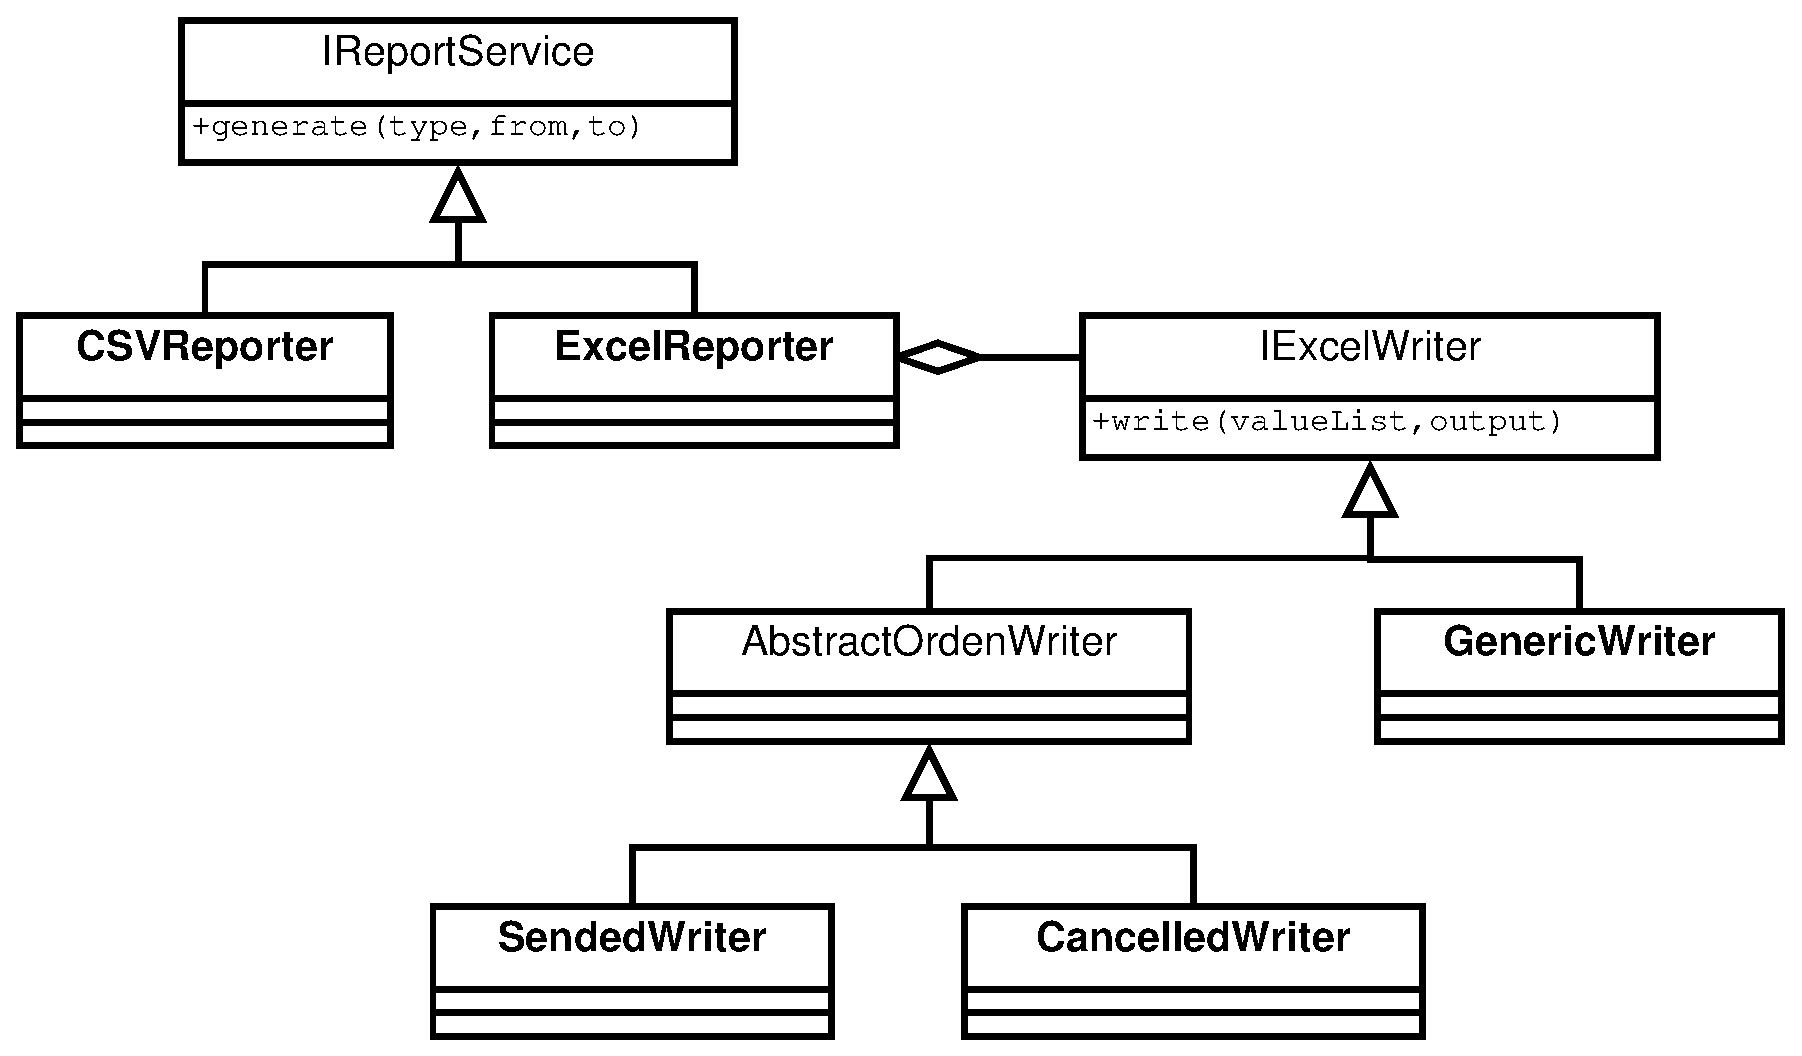
\includegraphics[scale=0.4]{dia-class-report-service}
	\caption{Diagrama de clases del servicio para generar reportes.}
	\label{fig:dia-class-report-service}
\end{figure}

\begin{enumerate}
	\item \textbf{IReportService}: el punto de entrada a la generación de reportes, define el método para la generación de los mismos que tiene como parámetros:
	\begin{itemize}
	 	\item \textbf{type}: tipo de reporte.
	 	\item \textbf{start}: fecha de inicio, acota la búsqueda de las órdenes de reposición únicamente incluyendo aquellas órdenes que hayan sido atendidas después de tal fecha.
	 	\item \textbf{end}: fecha de término, acota la búsqueda de las órdenes de reposición únicamente incluyendo aquellas órdenes que hayan sido atendidas antes de tal fecha.
	 \end{itemize}
	\item \textbf{CSVReporter}: Es la implementación específica de la generación de reportes en formato CSV.
	\item \textbf{ExcelReporter}: Es la implementación específica de la generación de reportes en formato Excel\textsuperscript{\textcopyright}.
	\item \textbf{IExcelWriter}: Describe la escritura de un registro en formato Excel\textsuperscript{\textcopyright}.
	\item \textbf{GenericWriter}: Escribe en forma genérica un registro, esto es, los valores son escritos en el orden que llegan sin ningún tratamiento extra. 
	\item \textbf{AbstractOrdenWriter}: Describe como escribir una orden de reposición a formato Excel\textsuperscript{\textcopyright}.
	\item \textbf{SendedWriter}: Esta clase se especializa en escribir órdenes de reposición que han sido atendidas.
	\item \textbf{CancelledWriter}: Esta clase se especializa en escribir órdenes de reposición que han sido canceladas.
\end{enumerate}



